% Template LaTeX untuk Ujian Kualifikasi
% Program Studi Doktor Informatika
% Universitas Telkom

% Document Class
\documentclass[12pt,a4paper]{article}

% Packages
\usepackage[utf8]{inputenc}
\usepackage[T1]{fontenc}
\usepackage{mathptmx} % Times New Roman
\usepackage{courier}  % Courier for monospace
\usepackage{helvet}   % Helvetica for sans-serif
\usepackage{amsmath}
\usepackage{geometry}
\usepackage{setspace}
\usepackage{titlesec}
\usepackage{graphicx}
\usepackage{hyperref}
\usepackage{booktabs}
\usepackage{array}
\usepackage[format=hang,font=footnotesize,labelfont=bf]{caption}
\usepackage{enumitem}
\usepackage{parskip}
\usepackage{fancyhdr}
\usepackage{tocloft}
\usepackage{tabularx}
\usepackage{longtable}
\usepackage{ragged2e}  % For better text justification in bibliography

% Page Setup
\geometry{
    top=3cm,
    bottom=3cm,
    left=4cm,
    right=3cm
}

% Title Formatting
\titleformat{\section}
    {\normalfont\fontsize{16}{19}\bfseries\centering}{\thesection}{1em}{}
    
\titleformat{\subsection}
    {\normalfont\fontsize{12}{14}\bfseries}{\thesubsection}{1em}{}

\titleformat{\subsubsection}
    {\normalfont\fontsize{12}{14}\normalfont}{\thesubsubsection}{1em}{}

% Spacing
\onehalfspacing

% Header/Footer
\pagestyle{fancy}
\fancyhf{}
\fancyfoot[C]{\thepage}
\renewcommand{\headrulewidth}{0pt}

% Hyperref setup
\hypersetup{
    colorlinks=true,
    linkcolor=black,
    citecolor=black,
    filecolor=black,
    urlcolor=black,
}

% Table of Contents customization
\renewcommand{\contentsname}{DAFTAR ISI}
\renewcommand{\cfttoctitlefont}{\hfill\fontsize{16}{19}\selectfont\bfseries}
\renewcommand{\cftaftertoctitle}{\hfill}

% List of Tables customization
\renewcommand{\listtablename}{DAFTAR TABEL}
\renewcommand{\cftlottitlefont}{\hfill\fontsize{16}{19}\selectfont\bfseries}
\renewcommand{\cftafterlottitle}{\hfill}

% List of Figures customization
\renewcommand{\listfigurename}{DAFTAR GAMBAR}
\renewcommand{\cftloftitlefont}{\hfill\fontsize{16}{19}\selectfont\bfseries}
\renewcommand{\cftafterloftitle}{\hfill}

% List of Equations setup
\newcommand{\listequationsname}{DAFTAR RUMUS}
\newlistof{myequations}{equ}{\listequationsname}
\newcommand{\myequations}[1]{%
\addcontentsline{equ}{myequations}{\protect\numberline{\theequation}#1}\par}
\renewcommand{\cftequtitlefont}{\hfill\fontsize{16}{19}\selectfont\bfseries}
\renewcommand{\cftafterequtitle}{\hfill}
\setlength{\cftmyequationsindent}{0pt}

% Redefine \listofequations to use the custom list
\newcommand{\listofequations}{\listofmyequations}

% Subsection numbering format
\renewcommand{\thesubsection}{\arabic{section}.\arabic{subsection}}

% Custom Commands
\newcommand{\myTitle}[1]{\def\@myTitle{#1}}
\newcommand{\myAuthorOne}[2]{\def\@myNameOne{#1}\def\@myNIMOne{#2}}
\newcommand{\myAuthorTwo}[2]{\def\@myNameTwo{#1}\def\@myNIMTwo{#2}}
\newcommand{\myYear}[1]{\def\@myYear{#1}}

% Redefine title
\makeatletter
% Initialize default values
\def\@myTitle{IMPLEMENTASI SISTEM POS BERBASIS WEB UNTUK OPTIMALISASI EFISIENSI OPERASIONAL PADA USAHA LAUNDRY}
\def\@myNameOne{Ismi Nabilah}
\def\@myNIMOne{714240056}
\def\@myNameTwo{Alifya Azzahra}
\def\@myNIMTwo{714240011}
\def\@myYear{2026}

\renewcommand{\maketitle}{
    \begin{titlepage}
        \centering
        \vspace*{0.5cm}
        
        % Judul Penelitian
        {\fontsize{14}{16}\selectfont\bfseries
        \@myTitle\par}
        
        \vspace{1.5cm}
        
        % Jenis Laporan
        {\fontsize{12}{14}\selectfont
        \textbf{LAPORAN PROYEK II}\par}
        \vspace{0.5cm}
        {\fontsize{12}{14}\selectfont
        Diajukan untuk Memenuhi Kelulusan Matakuliah Proyek 2 pada Program Studi DIV Teknik Informatika\par}
        
        \vspace{1.5cm}
        
        % Logo
        \IfFileExists{logo.png}{
            \includegraphics[width=0.4\textwidth]{logo.png}
        }{
            {\fontsize{16}{19}\bfseries Logo\par}
        }

        \vspace{1.5cm}
        
        % Penulis
        {\fontsize{12}{14}\selectfont
        \textbf{DISUSUN OLEH :}\par}
        \vspace{0.5cm}
        
        \begin{tabular}{ll}
            \textbf{\@myNIMOne} & \textbf{\@myNameOne} \\
            \textbf{\@myNIMTwo} & \textbf{\@myNameTwo}
        \end{tabular}\par
        
        \vfill
        
        % Program Studi dan Informasi
        {\fontsize{14}{16}\selectfont\bfseries
        PROGRAM STUDI DIV TEKNIK INFORMATIKA\par
        SEKOLAH VOKASI\par
        UNIVERSITAS LOGISTIK DAN BISNIS INTERNASIONAL\par
        BANDUNG\par
        \@myYear\par}
        
    \end{titlepage}
    \newpage
}
\makeatother

% Set Metadata
\myTitle{IMPLEMENTASI SISTEM POS BERBASIS WEB UNTUK OPTIMALISASI EFISIENSI OPERASIONAL PADA USAHA LAUNDRY}
\myAuthorOne{Ismi Nabilah}{714240056}
\myAuthorTwo{Alifya Azzahra}{714240011}
\myYear{2026}

% SOTA Table Environment
\newenvironment{sototable}
    {\begin{table}[htbp]
    \centering
    \caption{State-of-the-Art Penelitian}
    \label{tab:sota}}
    {\end{table}}

% Word Count Environments
\newenvironment{summary}
    {}
    {}

\newenvironment{background}
    {}
    {}

\newenvironment{literaturereview}
    {}
    {}

\newenvironment{researchgap}
    {}
    {}

\newenvironment{novelty}
    {}
    {}

% Bibliography Style - APA-like with BibTeX
\usepackage[
    backend=bibtex,   % Menggunakan BibTeX (biber tidak berfungsi di sistem ini)
    style=authoryear, % Author-year citation style (APA-like)
    sorting=nyt,      % Sort by name, year, title
    maxbibnames=99,   % Tampilkan semua nama penulis
    dashed=false,     % Jangan gunakan dash untuk author yang sama
    url=false,        % Jangan tampilkan URL
    doi=true,         % Tampilkan DOI
]{biblatex}

\urlstyle{same} % Samakan font URL/DOI dengan teks utama

\addbibresource{references.bib}
\addbibresource{include.bib}
%\addbibresource{visualdecoding.bib} % Uncomment jika ingin menggunakan file bib tambahan

% Make \cite behave like \parencite (with parentheses)
\let\cite\parencite

% Custom citation formatting
\renewcommand*{\finalnamedelim}{\addspace\&\addspace}  % Ubah "and" jadi "&"
\renewcommand*{\nameyeardelim}{\addcomma\space}        % Tambahkan koma setelah author

% Remove "In:" from bibliography
\renewbibmacro{in:}{}

% Ensure pages are not bold
\DeclareFieldFormat{pages}{\normalfont #1}

% Custom format untuk memastikan ada spasi setelah "in"
\DeclareFieldFormat{booktitle}{\addspace\textit{#1}}
\DeclareFieldFormat{journaltitle}{\addspace\textit{#1}}

% Fix URL breaking untuk mencegah overflow
\setcounter{biburllcpenalty}{7000}
\setcounter{biburlucpenalty}{8000}

% Set bibliography to use ragged right alignment untuk mencegah overfull
\emergencystretch=1em
\appto{\bibsetup}{\sloppy\RaggedRight}



% Set document metadata (sudah dipindahkan ke baris 170-173, hapus duplikat ini)
% \myTitle{IMPLEMENTASI SISTEM POS BERBASIS WEB UNTUK OPTIMALISASI EFISIENSI OPERASIONAL PADA USAHA LAUNDRY}
% \myAuthorOne{Ismi Nabilah}{714240056}
% \myAuthorTwo{Alifya Azzahra}{714240011}
% \myYear{2026}

% Beginning of Document
\begin{document}

% Force TOC title to be uppercase (fix for babel override)
\renewcommand{\contentsname}{DAFTAR ISI}
\renewcommand{\listtablename}{DAFTAR TABEL}
\renewcommand{\listfigurename}{DAFTAR GAMBAR}

% Use Times New Roman as default font
\rmfamily

% Title Page
\maketitle

% Halaman Depan menggunakan angka Romawi
\pagenumbering{roman}

% DAFTAR ISI
\phantomsection
\addcontentsline{toc}{section}{DAFTAR ISI}
\tableofcontents
\clearpage

% DAFTAR TABEL
\phantomsection
\addcontentsline{toc}{section}{DAFTAR TABEL}
\listoftables
\clearpage

% DAFTAR GAMBAR
\phantomsection
\addcontentsline{toc}{section}{DAFTAR GAMBAR}
\listoffigures
\clearpage

% DAFTAR RUMUS
\phantomsection
\addcontentsline{toc}{section}{DAFTAR RUMUS}
\listofequations
\clearpage

% RINGKASAN
\clearpage
\section*{RINGKASAN}
\phantomsection
\addcontentsline{toc}{section}{RINGKASAN}
\input{chapters/ringkasan}

\clearpage

% BAB 1 - PENDAHULUAN
\setcounter{section}{0}
\pagenumbering{arabic} % Kembali ke angka Arab mulai dari Bab 1
\setcounter{page}{1}   % Reset halaman ke 1
\section*{BAB 1 \\ PENDAHULUAN}
\phantomsection
\addcontentsline{toc}{section}{BAB 1 PENDAHULUAN}
\refstepcounter{section}

% BAB 1 - PENDAHULUAN

\vspace{1cm}
\subsection{Deskripsi Aplikasi}
\indent
Perkembangan teknologi informasi mendorong usaha kecil, termasuk laundry, untuk beralih dari pencatatan konvensional ke sistem digital. Salah satu solusi yang dikembangkan adalah Sistem Point of Sale (POS) Laundry berbasis web, yang berfungsi untuk mencatat transaksi, mengelola data pelanggan, memantau status cucian, serta menyusun laporan operasional secara terintegrasi. Dengan berbasis web, sistem ini dapat diakses secara fleksibel dari berbagai perangkat, sehingga meningkatkan efisiensi dan memudahkan pemilik usaha dalam melakukan monitoring \cite{Achyani2024}.

Penelitian sebelumnya menegaskan bahwa aplikasi laundry berbasis web mampu menyederhanakan proses pencarian dan pengelolaan layanan laundry, sekaligus meningkatkan transparansi data dan akurasi pencatatan \cite{Singh2022}. Selain itu, pendekatan berbasis pengguna dalam pengembangan sistem laundry terbukti dapat memperbaiki alur operasional dan meningkatkan kepuasan pelanggan, terutama melalui antarmuka yang mudah digunakan dan proses transaksi yang lebih cepat \cite{Kalo2023}.

Studi lokal juga menunjukkan bahwa sistem informasi laundry berbasis web dapat membantu pemilik usaha dalam mengurangi kesalahan pencatatan, mempercepat proses transaksi, serta menghasilkan laporan yang lebih rapi dan terstruktur \cite{SigitSugiharto2023}. Penelitian lain menekankan bahwa penerapan sistem digital pada usaha kecil menengah (UMKM) berpengaruh positif terhadap efisiensi operasional dan kualitas layanan, sehingga mendukung keberlanjutan bisnis \cite{Maulana2025}.

Berdasarkan kondisi tersebut, usaha laundry yang masih bergantung pada pencatatan berbasis kertas berisiko menghadapi kendala seperti kesalahan hitung, keterlambatan informasi, dan pengelolaan data yang kurang optimal. Oleh karena itu, pengembangan Sistem POS Laundry Berbasis Website diharapkan menjadi solusi yang mampu meningkatkan efisiensi operasional, kualitas layanan, serta kepuasan pelanggan secara berkelanjutan.

\subsection{Identifikasi Masalah}
\noindent
Berdasarkan latar belakang yang telah dijelaskan, maka pertanyaan penelitian (\textit{research questions}) yang diidentifikasi dalam penelitian ini adalah sebagai berikut:

\begin{enumerate}
    \item Bagaimana merancang sistem POS Laundry berbasis web yang mampu mentransformasi pencatatan konvensional menjadi sistem informasi yang terintegrasi?
    \item Bagaimana mengimplementasikan mekanisme \textit{callback} notifikasi pembayaran QRIS untuk mengautomasi verifikasi transaksi secara \textit{real-time}?
    \item Bagaimana menjamin keandalan fitur pembayaran digital pada sistem menggunakan pengujian unit dengan target 100\% \textit{statement coverage}?
    \item Bagaimana penerapan metode Scrum dapat mendukung pengembangan sistem yang adaptif terhadap kebutuhan operasional UMKM Laundry?
\end{enumerate}

\noindent
Pertanyaan penelitian ini dirumuskan untuk menjawab kebutuhan akan sistem yang tidak hanya mendigitalisasi data, tetapi juga membawa pembaruan pada aspek automasi dan validasi data transaksi \cite{Achyani2024,Mutia2025}.

\subsection{Tujuan}
\noindent
Tujuan dari penelitian dan pengembangan sistem POS Laundry berbasis web ini adalah:

\begin{enumerate}
    \item Merancang dan membangun sistem POS Laundry berbasis web yang terintegrasi untuk meningkatkan efisiensi operasional.
    \item Membangun fitur automasi verifikasi pembayaran QRIS yang mampu mendeteksi dana masuk secara otomatis guna meminimalkan celah manipulasi data.
    \item Mencapai tingkat \textit{statement coverage} sebesar 100\% pada modul krusial untuk memastikan sistem bebas dari kesalahan logika.
    \item Mengoptimalkan pengelolaan data pelanggan dan laporan keuangan melalui basis data yang terstruktur.
\end{enumerate}

\noindent
Tujuan ini didukung oleh penelitian sebelumnya yang menunjukkan bahwa sistem berbasis web dapat meningkatkan efisiensi operasional, memperbaiki kualitas layanan, dan mendukung keberlanjutan usaha laundry \cite{Achyani2024,Kalo2023,SigitSugiharto2023,Maulana2025}.

\subsection{Lingkup Dokumentasi}
\noindent
Lingkup dokumentasi pada proyek ini dibatasi pada aspek-aspek utama yang mendukung pengembangan Sistem POS Laundry berbasis web, meliputi:

\begin{enumerate}
    \item Analisis kebutuhan sistem yang mencakup identifikasi modul inti seperti transaksi, pelanggan, dan laporan.
    \item Perancangan sistem berbasis web yang meliputi desain antarmuka sederhana, responsif, dan mudah digunakan.
    \item Implementasi modul inti berupa transaksi laundry, manajemen pelanggan, serta laporan operasional dan keuangan.
    \item Evaluasi awal sistem melalui uji coba terbatas untuk menilai efisiensi dan akurasi pencatatan.
\end{enumerate}

\noindent
Batasan dokumentasi tidak mencakup pengembangan aplikasi mobile, integrasi notifikasi otomatis, maupun fitur tambahan di luar modul inti. Fokus diarahkan pada sistem berbasis web yang mendukung pencatatan transaksi, pemantauan status cucian, dan penyusunan laporan secara terstruktur \cite{Mutia2025,Lizal2025,Kalo2023}.


\clearpage

% BAB 2 - LITERATURE REVIEW
\section*{BAB 2 \\ LITERATURE REVIEW}
\phantomsection
\addcontentsline{toc}{section}{BAB 2 LITERATURE REVIEW}
\refstepcounter{section}

% BAB 2 - LANDASAN TEORI

% Ganti dengan konten dari laporan Word kamu
% Biasanya berisi teori-teori yang relevan dengan penelitian

\subsection{Sistem Informasi}
\indent
Sistem informasi adalah kombinasi dari teknologi, manusia, dan prosedur yang digunakan untuk mengumpulkan, memproses, menyimpan, serta mendistribusikan informasi guna mendukung pengambilan keputusan dan koordinasi dalam organisasi. Menurut Laudon & Laudon dalam Management Information Systems: Managing the Digital Firm (2021), sistem informasi berperan penting dalam meningkatkan efisiensi operasional dan kualitas layanan melalui integrasi data dan proses bisnis. Hal ini sejalan dengan O’Brien dalam Introduction to Information Systems (2004) yang menekankan bahwa sistem informasi modern tidak hanya berfungsi sebagai alat pencatatan, tetapi juga sebagai sarana strategis untuk mendukung keberlangsungan bisnis di era digital. Dalam konteks modern, sistem informasi berbasis web menjadi pilihan utama karena dapat diakses secara fleksibel melalui berbagai perangkat, sehingga mendukung transparansi data dan integrasi proses bisnis [8][9].

\subsection{Poin of Sale (POS)}
\indent
Point of Sale (POS) adalah sistem yang digunakan untuk mencatat transaksi penjualan secara digital dan terintegrasi. POS tidak hanya berfungsi sebagai alat pencatatan, tetapi juga sebagai sistem manajemen yang mampu menghubungkan data transaksi dengan laporan keuangan dan inventori. POS berbasis web memiliki keunggulan dibandingkan POS tradisional karena memungkinkan akses multi device, integrasi data secara real time, serta mempermudah pemilik usaha dalam melakukan monitoring. Penelitian menunjukkan bahwa sistem berbasis web dapat meningkatkan akurasi pencatatan dan efisiensi operasional [1][2]

\subsection{Usaha Laundry}
\indent
Usaha laundry sebagai bagian dari UMKM sering menghadapi kendala dalam pencatatan manual, seperti kesalahan transaksi, keterlambatan informasi, dan laporan yang tidak terstruktur. Digitalisasi layanan laundry melalui sistem POS berbasis web menjadi solusi untuk mengatasi permasalahan tersebut. Penelitian terdahulu menegaskan bahwa sistem laundry berbasis web mampu menyederhanakan proses pencatatan, mempercepat transaksi, serta meningkatkan kepuasan pelanggan melalui antarmuka yang mudah digunakan [3][4][5]. Studi lain juga menekankan bahwa digitalisasi laundry mendukung keberlanjutan usaha kecil dengan menyediakan laporan yang lebih rapi dan terstruktur [6][7].

\subsection{Teori Usability dan User Experience}
\indent
Selain itu, teori usability menurut ISO 9241 11 menekankan bahwa sistem harus memenuhi aspek efektivitas, efisiensi, dan kepuasan pengguna. Prinsip usability sangat relevan dalam pengembangan POS Laundry berbasis web, karena antarmuka yang sederhana dan informatif akan mempermudah karyawan maupun pemilik dalam menggunakan sistem. Dengan demikian, pengembangan sistem POS Laundry berbasis web tidak hanya didukung oleh konsep sistem informasi dan POS, tetapi juga oleh teori usability yang memastikan sistem dapat digunakan secara optimal oleh penggunanya [3].
% Tambahkan subsection lain sesuai kebutuhan


\clearpage

% BAB 3 - TEORI / METODE TERKAIT
\section*{BAB 3 \\ TEORI / METODE TERKAIT}
\phantomsection
\addcontentsline{toc}{section}{BAB 3 TEORI / METODE TERKAIT}
\refstepcounter{section}

% BAB 3 - ANALISIS PERANCANGAN

% Ganti dengan konten dari laporan Word kamu
% Biasanya berisi analisis sistem dan perancangan

\subsection{Analisis}
\subsubsection{Analisis Fungsi Fungsional}
\indent
Analisis fungsional dilakukan untuk mengidentifikasi kebutuhan utama sistem POS Laundry berbasis web. Sistem ini dirancang agar dapat menggantikan pencatatan manual dengan menyediakan fitur inti sebagai berikut:

\begin{itemize}
    \item Transaksi Laundry: mencatat pesanan pelanggan, jenis layanan (cuci, setrika, paket), jumlah, harga, dan status cucian.
    \item Manajemen Pelanggan: menyimpan data pelanggan, riwayat transaksi, serta mempermudah pencarian informasi.
    \item Laporan Operasional dan Keuangan: menghasilkan laporan harian, mingguan, dan bulanan terkait jumlah transaksi, pendapatan, serta status cucian.
    \item Pengelolaan Status Cucian: menampilkan status cucian (proses, selesai, diambil) secara real time.
\end{itemize}

\noindent
Fungsi fungsi ini mendukung tujuan sistem untuk meningkatkan efisiensi, akurasi pencatatan, dan transparansi layanan.


\subsubsection{Analisis Non Fungsional}
\indent
Selain kebutuhan fungsional, sistem juga harus memenuhi kebutuhan non fungsional agar dapat digunakan secara optimal:

\begin{itemize}
    \item Keamanan Data: sistem harus melindungi data pelanggan dan transaksi dari akses tidak sah.
    \item Kinerja Sistem: aplikasi harus mampu memproses transaksi dengan cepat dan stabil.
    \item Usability: antarmuka harus sederhana, responsif, dan mudah dipahami oleh karyawan maupun pemilik.
    \item Portabilitas: sistem berbasis web dapat diakses melalui berbagai perangkat (PC, laptop, smartphone).
    \item Reliabilitas: sistem harus mampu beroperasi secara konsisten tanpa gangguan yang signifikan.
\end{itemize}


\subsection{Perancangan}
\indent
Tahap perancangan merupakan proses penerjemahan hasil analisis kebutuhan ke dalam bentuk rancangan teknis yang akan digunakan sebagai acuan dalam pengembangan sistem POS Laundry berbasis web. Perancangan ini mencakup struktur menu, desain antarmuka pengguna, perancangan basis data, serta logika fungsi yang mendukung operasional laundry secara digital.

\indent
Tujuan utama dari perancangan adalah memastikan bahwa sistem yang dibangun sesuai dengan kebutuhan fungsional dan non fungsional yang telah diidentifikasi sebelumnya. Dengan rancangan yang terstruktur, pengembangan sistem dapat dilakukan secara efisien, terarah, dan minim risiko kesalahan implementasi. Setiap komponen yang dirancang baik dari sisi tampilan maupun proses internal harus mampu mendukung pencatatan transaksi, pengelolaan pelanggan, dan penyusunan laporan secara akurat dan real time.


\subsubsection{Usecase Diagram}
[gambar usecase]


\subsubsection{Antarmuka (UI)}
\indent
Desain antarmuka yang dirancang menggunakan prinsip responsif dan sederhana agar mudah digunakan oleh pengguna, baik melalui komputer maupun smartphone. Berdasarkan analisis kebutuhan, berikut adalah komponen utama dari antarmuka yang dirancang:

\begin{enumerate}
    \item Halaman Login: Proses login melibatkan pengisian formulir terautentikasi untuk mendapatkan akses ke sistem yang memisahkan administrator dan pengguna.
    \item Dashboard Admin: Area admin utama dengan menu navigasi untuk melihat data pengguna, data laundry, dan ringkasan laporan keuangan serta kinerja bisnis.
    \item Dashboard Kasir: Ruang kerja utama untuk Kasir yang menyediakan fitur cepat untuk memasukkan transaksi baru, memeriksa status pelanggan, dan menganalisis data pelanggan.
    \item Halaman Transaksi: Antarmuka untuk menentukan jenis layanan laundry (kiloan/satuan), menghitung total biaya secara otomatis, dan memproses pembayaran.
    \item truk Transaksi:Tampilan bukti pembayaran yang dapat dicetak atau dikirim secara digital kepada pelanggan berisi detail layanan dan total biaya.
\end{enumerate}


\subsubsection{Struktur Database}
[gambar]

\indent
Berdasarkan gambar 3.2.3 diatas, sistem ini menggunakan tiga tabel utama yang saling berelasi untuk mengelola data operasional laundry:

\begin{enumerate}
    \item Tabel Pelanggan. Digunakan untuk menyimpan informasi identitas pelanggan seperti nama, alamat, telepon.
    \item Tabel Layanan. Berisi daftar jenis jasa laundry yang ditawarkan, termasuk informasi seperti nama layanan, harga, satuan (misalnya per kg atau per potong), dan deskripsi.
    \item Tabel Transaksi. Mencatat setiap pesanan yang dilakukan oleh pelanggan, termasuk total (biaya), status (status pengerjaan/pembayaran), dan berat (untuk laundry kiloan).
\end{enumerate}


\subsubsection{Algoritma fungsi}
\indent
Dalam pengembangan sistem point-of-sale laundry berbasis web ini, algoritma fungsional digunakan untuk menentukan logika bisnis utama, seperti total biaya berdasarkan berat atau kuantitas, pemantauan status cucian secara real-time, dan laporan keuangan otomatis. Algoritma ini digunakan untuk memastikan proses kerja sistematis, akurat, dan meminimalkan kesulitan yang terkait dengan pekerjaan manual.

\subsubsection{Flowchart}
[gambar]

% DAFTAR PUSTAKA
\clearpage
\section*{DAFTAR PUSTAKA}
\phantomsection
\addcontentsline{toc}{section}{DAFTAR PUSTAKA}

\printbibliography[heading=none]

\clearpage


\clearpage
\section*{LAMPIRAN}
\phantomsection
\addcontentsline{toc}{section}{LAMPIRAN}

% 1. Reset penomoran gambar agar dimulai dari L.1, L.2, dst.
\setcounter{figure}{0} 
\renewcommand{\thefigure}{L.\arabic{figure}}

% 2. Pastikan label yang muncul adalah "Gambar", bukan "Figure"
\renewcommand{\figurename}{Gambar}

\vspace{1cm}
\noindent
\textbf{HASIL PENGUJIAN UNIT (UNIT TESTING)}

\noindent
Lampiran ini menyajikan data teknis hasil audit pengujian unit yang dilakukan terhadap seluruh fungsionalitas backend Sistem POS WellClean Laundry menggunakan tool \texttt{go tool cover}. Pengujian ini memvalidasi integritas logika baris kode pada setiap fungsi utama.

\begin{figure}[H]
    \centering
    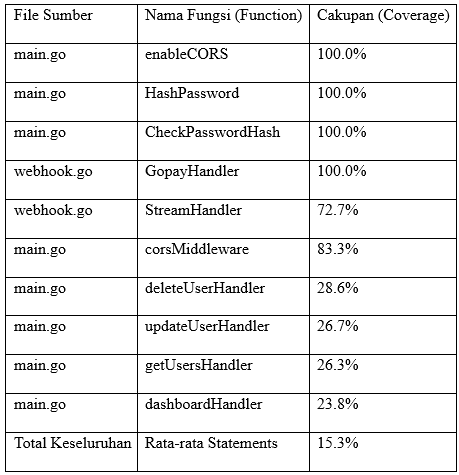
\includegraphics[width=0.8\textwidth]{images/rekapitulasi.png}
    \caption{Rekapitulasi Cakupan Baris Kode (Statements)}
    \label{fig:rekapitulasi}
\end{figure}

\begin{figure}[H]
    \centering
    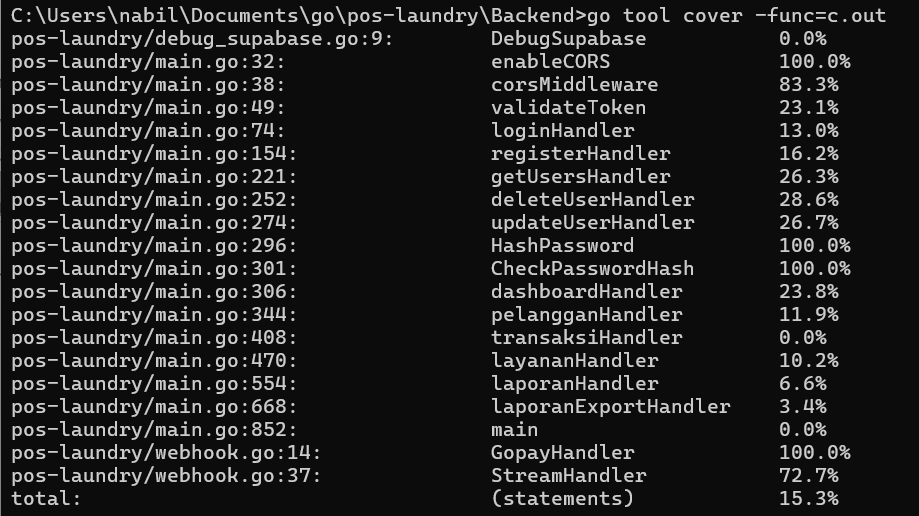
\includegraphics[width=0.8\textwidth]{images/codecoverage.png}
    \caption{Tangkapan Layar Hasil Codecoverage}
    \label{fig:codecoverage}
\end{figure}

\clearpage

\end{document}
